\documentclass{book}
\usepackage[a4paper,top=2.5cm,bottom=2.5cm,left=2.5cm,right=2.5cm]{geometry}
\usepackage{makeidx}
\usepackage{natbib}
\usepackage{graphicx}
\usepackage{multicol}
\usepackage{float}
\usepackage{listings}
\usepackage{color}
\usepackage{ifthen}
\usepackage[table]{xcolor}
\usepackage{textcomp}
\usepackage{alltt}
\usepackage{ifpdf}
\ifpdf
\usepackage[pdftex,
            pagebackref=true,
            colorlinks=true,
            linkcolor=blue,
            unicode
           ]{hyperref}
\else
\usepackage[ps2pdf,
            pagebackref=true,
            colorlinks=true,
            linkcolor=blue,
            unicode
           ]{hyperref}
\usepackage{pspicture}
\fi
\usepackage[utf8]{inputenc}
\usepackage{mathptmx}
\usepackage[scaled=.90]{helvet}
\usepackage{courier}
\usepackage{sectsty}
\usepackage{amssymb}
\usepackage[titles]{tocloft}
\usepackage{doxygen}
\lstset{language=C++,inputencoding=utf8,basicstyle=\footnotesize,breaklines=true,breakatwhitespace=true,tabsize=8,numbers=left }
\makeindex
\setcounter{tocdepth}{3}
\renewcommand{\footrulewidth}{0.4pt}
\renewcommand{\familydefault}{\sfdefault}
\hfuzz=15pt
\setlength{\emergencystretch}{15pt}
\hbadness=750
\tolerance=750
\begin{document}
\hypersetup{pageanchor=false,citecolor=blue}
\begin{titlepage}
\vspace*{7cm}
\begin{center}
{\Large My Project }\\
\vspace*{1cm}
{\large Generated by Doxygen 1.8.1.2}\\
\vspace*{0.5cm}
{\small Wed Jun 25 2014 19:32:54}\\
\end{center}
\end{titlepage}
\clearemptydoublepage
\pagenumbering{roman}
\tableofcontents
\clearemptydoublepage
\pagenumbering{arabic}
\hypersetup{pageanchor=true,citecolor=blue}
\chapter{Class Index}
\section{Class Hierarchy}
This inheritance list is sorted roughly, but not completely, alphabetically\+:\begin{DoxyCompactList}
\item \contentsline{section}{Animal}{\pageref{class_animal}}{}
\begin{DoxyCompactList}
\item \contentsline{section}{Cat}{\pageref{class_cat}}{}
\item \contentsline{section}{Dog}{\pageref{class_dog}}{}
\end{DoxyCompactList}
\item object\begin{DoxyCompactList}
\item \contentsline{section}{doxygen\+\_\+python.\+Sample\+Class}{\pageref{classdoxygen__python_1_1_sample_class}}{}
\end{DoxyCompactList}
\item \contentsline{section}{test.\+Staterobot}{\pageref{classtest_1_1_staterobot}}{}
\begin{DoxyCompactList}
\item \contentsline{section}{test.\+testing}{\pageref{classtest_1_1testing}}{}
\end{DoxyCompactList}
\end{DoxyCompactList}

\chapter{Class Index}
\section{Class List}
Here are the classes, structs, unions and interfaces with brief descriptions\-:\begin{DoxyCompactList}
\item\contentsline{section}{\hyperlink{class_animal}{Animal} }{\pageref{class_animal}}{}
\item\contentsline{section}{\hyperlink{class_cat}{Cat} }{\pageref{class_cat}}{}
\item\contentsline{section}{\hyperlink{class_dog}{Dog} }{\pageref{class_dog}}{}
\item\contentsline{section}{\hyperlink{classtest_1_1_staterobot}{test.\-Staterobot} }{\pageref{classtest_1_1_staterobot}}{}
\item\contentsline{section}{\hyperlink{classtest_1_1testing}{test.\-testing} }{\pageref{classtest_1_1testing}}{}
\end{DoxyCompactList}

\chapter{Class Documentation}
\hypertarget{class_animal}{\section{Animal Class Reference}
\label{class_animal}\index{Animal@{Animal}}
}


Inheritance diagram for Animal\-:
\nopagebreak
\begin{figure}[H]
\begin{center}
\leavevmode
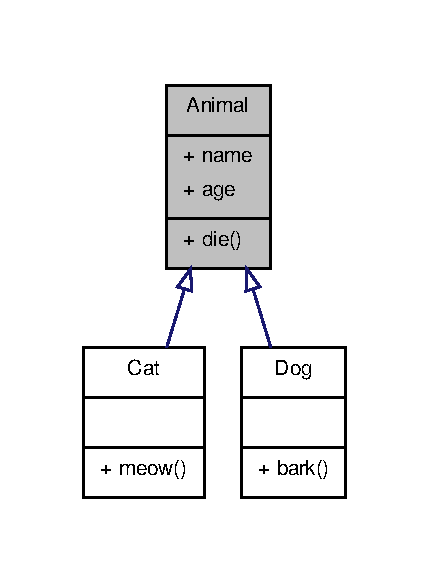
\includegraphics[width=206pt]{class_animal__inherit__graph}
\end{center}
\end{figure}


Collaboration diagram for Animal\-:
\nopagebreak
\begin{figure}[H]
\begin{center}
\leavevmode
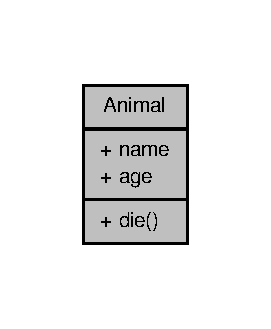
\includegraphics[width=130pt]{class_animal__coll__graph}
\end{center}
\end{figure}
\subsection*{Public Member Functions}
\begin{DoxyCompactItemize}
\item 
\hypertarget{class_animal_a557fe0d71dda75be2f8459ce0d7c2275}{void {\bfseries die} ()}\label{class_animal_a557fe0d71dda75be2f8459ce0d7c2275}

\end{DoxyCompactItemize}
\subsection*{Public Attributes}
\begin{DoxyCompactItemize}
\item 
\hypertarget{class_animal_a9cf3bfd9070daec7b3bbc87cbd958f35}{string {\bfseries name}}\label{class_animal_a9cf3bfd9070daec7b3bbc87cbd958f35}

\item 
\hypertarget{class_animal_a31e4a23bef9596927496de4eb6b9c721}{int {\bfseries age}}\label{class_animal_a31e4a23bef9596927496de4eb6b9c721}

\end{DoxyCompactItemize}


The documentation for this class was generated from the following file\-:\begin{DoxyCompactItemize}
\item 
test.\-cpp\end{DoxyCompactItemize}

\hypertarget{class_cat}{\section{Cat Class Reference}
\label{class_cat}\index{Cat@{Cat}}
}


Inheritance diagram for Cat\+:\nopagebreak
\begin{figure}[H]
\begin{center}
\leavevmode
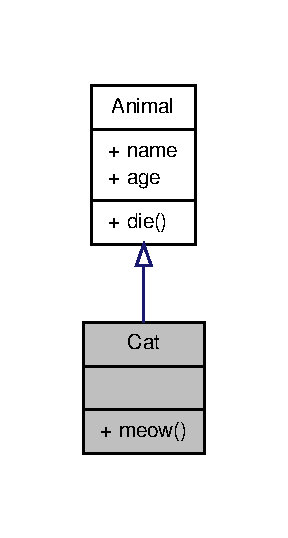
\includegraphics[width=138pt]{class_cat__inherit__graph}
\end{center}
\end{figure}


Collaboration diagram for Cat\+:\nopagebreak
\begin{figure}[H]
\begin{center}
\leavevmode
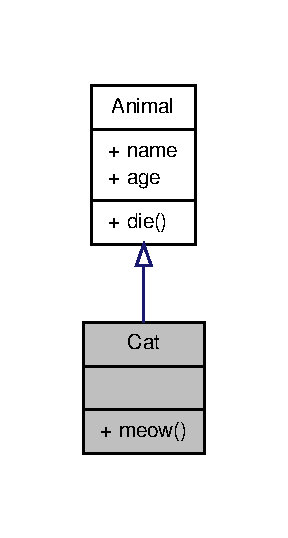
\includegraphics[width=138pt]{class_cat__coll__graph}
\end{center}
\end{figure}
\subsection*{Public Member Functions}
\begin{DoxyCompactItemize}
\item 
void \hyperlink{class_cat_aa770c672b7458b036d7384a6915d9367}{meow} ()
\end{DoxyCompactItemize}
\subsection*{Additional Inherited Members}


\subsection{Member Function Documentation}
\hypertarget{class_cat_aa770c672b7458b036d7384a6915d9367}{\index{Cat@{Cat}!meow@{meow}}
\index{meow@{meow}!Cat@{Cat}}
\subsubsection[{meow}]{\setlength{\rightskip}{0pt plus 5cm}void Cat\+::meow (
\begin{DoxyParamCaption}
{}
\end{DoxyParamCaption}
)}}\label{class_cat_aa770c672b7458b036d7384a6915d9367}


The documentation for this class was generated from the following file\+:\begin{DoxyCompactItemize}
\item 
\hyperlink{test_8cpp}{test.\+cpp}\end{DoxyCompactItemize}

\hypertarget{class_dog}{\section{Dog Class Reference}
\label{class_dog}\index{Dog@{Dog}}
}


Inheritance diagram for Dog\+:\nopagebreak
\begin{figure}[H]
\begin{center}
\leavevmode
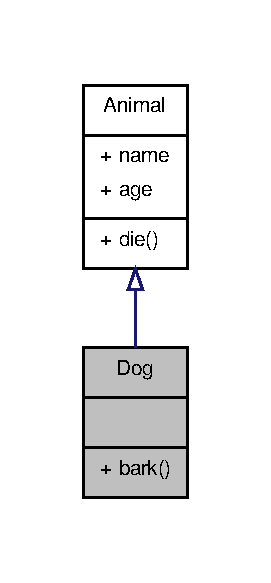
\includegraphics[width=130pt]{class_dog__inherit__graph}
\end{center}
\end{figure}


Collaboration diagram for Dog\+:\nopagebreak
\begin{figure}[H]
\begin{center}
\leavevmode
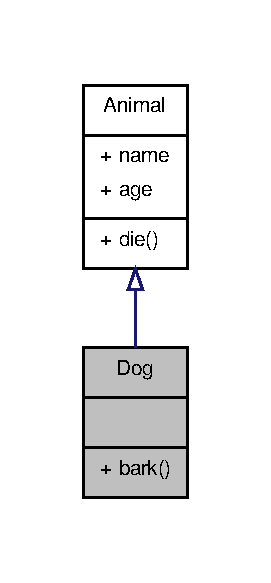
\includegraphics[width=130pt]{class_dog__coll__graph}
\end{center}
\end{figure}
\subsection*{Public Member Functions}
\begin{DoxyCompactItemize}
\item 
void \hyperlink{class_dog_ad3ab5661e3663948a486ff73049b1e1f}{bark} ()
\end{DoxyCompactItemize}
\subsection*{Additional Inherited Members}


\subsection{Member Function Documentation}
\hypertarget{class_dog_ad3ab5661e3663948a486ff73049b1e1f}{\index{Dog@{Dog}!bark@{bark}}
\index{bark@{bark}!Dog@{Dog}}
\subsubsection[{bark}]{\setlength{\rightskip}{0pt plus 5cm}void Dog\+::bark (
\begin{DoxyParamCaption}
{}
\end{DoxyParamCaption}
)}}\label{class_dog_ad3ab5661e3663948a486ff73049b1e1f}


The documentation for this class was generated from the following file\+:\begin{DoxyCompactItemize}
\item 
\hyperlink{test_8cpp}{test.\+cpp}\end{DoxyCompactItemize}

\hypertarget{classtest_1_1_staterobot}{\section{test.\-Staterobot Class Reference}
\label{classtest_1_1_staterobot}\index{test.\-Staterobot@{test.\-Staterobot}}
}


Inheritance diagram for test.\-Staterobot\-:
\nopagebreak
\begin{figure}[H]
\begin{center}
\leavevmode
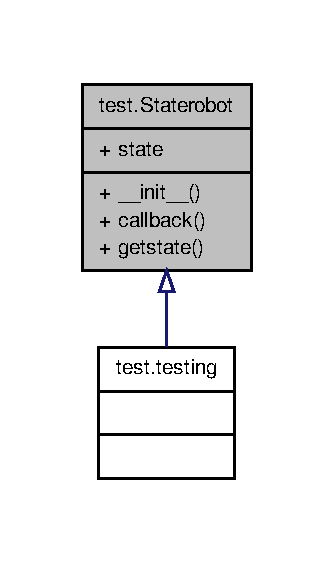
\includegraphics[width=160pt]{classtest_1_1_staterobot__inherit__graph}
\end{center}
\end{figure}


Collaboration diagram for test.\-Staterobot\-:
\nopagebreak
\begin{figure}[H]
\begin{center}
\leavevmode
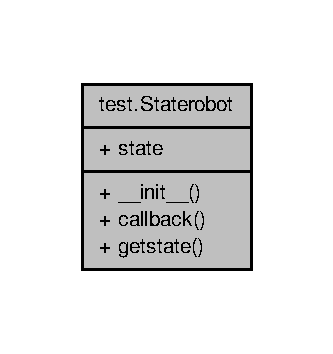
\includegraphics[width=160pt]{classtest_1_1_staterobot__coll__graph}
\end{center}
\end{figure}
\subsection*{Public Member Functions}
\begin{DoxyCompactItemize}
\item 
\hypertarget{classtest_1_1_staterobot_a825aa6cfc4a937fae93b18eb22d5049d}{def {\bfseries \-\_\-\-\_\-init\-\_\-\-\_\-}}\label{classtest_1_1_staterobot_a825aa6cfc4a937fae93b18eb22d5049d}

\item 
\hypertarget{classtest_1_1_staterobot_a2c8f2fc540f84bfc18477fdde6510bfa}{def {\bfseries callback}}\label{classtest_1_1_staterobot_a2c8f2fc540f84bfc18477fdde6510bfa}

\item 
\hypertarget{classtest_1_1_staterobot_a5663f3bcd6262303e19c4735396cbef2}{def {\bfseries getstate}}\label{classtest_1_1_staterobot_a5663f3bcd6262303e19c4735396cbef2}

\end{DoxyCompactItemize}
\subsection*{Public Attributes}
\begin{DoxyCompactItemize}
\item 
\hypertarget{classtest_1_1_staterobot_a6ac3890142e62ba6a4e96f3090fa9b38}{{\bfseries state}}\label{classtest_1_1_staterobot_a6ac3890142e62ba6a4e96f3090fa9b38}

\end{DoxyCompactItemize}


The documentation for this class was generated from the following file\-:\begin{DoxyCompactItemize}
\item 
test.\-py\end{DoxyCompactItemize}

\hypertarget{classtest_1_1testing}{\section{test.\-testing Class Reference}
\label{classtest_1_1testing}\index{test.\-testing@{test.\-testing}}
}


Inheritance diagram for test.\-testing\-:
\nopagebreak
\begin{figure}[H]
\begin{center}
\leavevmode
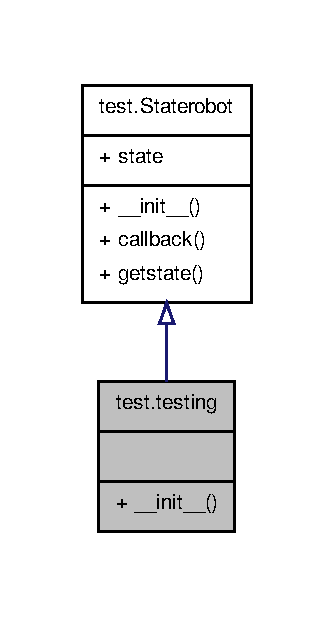
\includegraphics[width=160pt]{classtest_1_1testing__inherit__graph}
\end{center}
\end{figure}


Collaboration diagram for test.\-testing\-:
\nopagebreak
\begin{figure}[H]
\begin{center}
\leavevmode
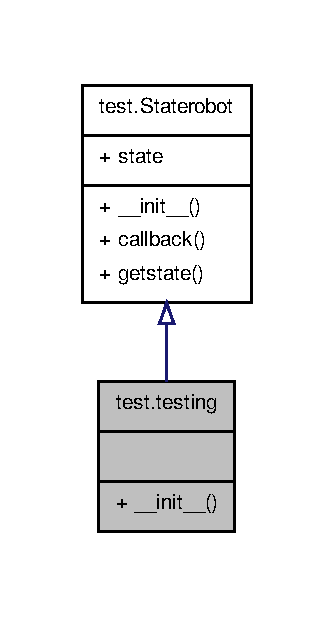
\includegraphics[width=160pt]{classtest_1_1testing__coll__graph}
\end{center}
\end{figure}
\subsection*{Additional Inherited Members}


The documentation for this class was generated from the following file\-:\begin{DoxyCompactItemize}
\item 
test.\-py\end{DoxyCompactItemize}

\printindex
\end{document}
